% Created by tikzDevice version 0.12
% !TEX encoding = UTF-8 Unicode
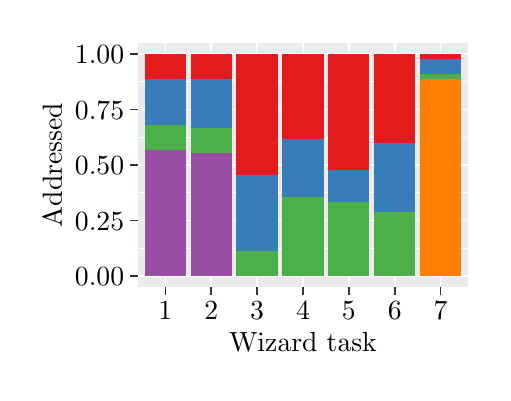
\begin{tikzpicture}[x=1pt,y=1pt]
\definecolor{fillColor}{RGB}{255,255,255}
\path[use as bounding box,fill=fillColor,fill opacity=0.00] (0,0) rectangle (164.64,124.59);
\begin{scope}
\path[clip] (  0.00,  0.00) rectangle (164.64,124.59);
\definecolor{drawColor}{RGB}{255,255,255}
\definecolor{fillColor}{RGB}{255,255,255}

\path[draw=drawColor,line width= 0.6pt,line join=round,line cap=round,fill=fillColor] (  0.00,  0.00) rectangle (164.64,124.59);
\end{scope}
\begin{scope}
\path[clip] ( 39.80, 30.86) rectangle (159.14,119.09);
\definecolor{fillColor}{gray}{0.92}

\path[fill=fillColor] ( 39.80, 30.86) rectangle (159.14,119.09);
\definecolor{drawColor}{RGB}{255,255,255}

\path[draw=drawColor,line width= 0.3pt,line join=round] ( 39.80, 44.90) --
	(159.14, 44.90);

\path[draw=drawColor,line width= 0.3pt,line join=round] ( 39.80, 64.95) --
	(159.14, 64.95);

\path[draw=drawColor,line width= 0.3pt,line join=round] ( 39.80, 85.00) --
	(159.14, 85.00);

\path[draw=drawColor,line width= 0.3pt,line join=round] ( 39.80,105.05) --
	(159.14,105.05);

\path[draw=drawColor,line width= 0.6pt,line join=round] ( 39.80, 34.87) --
	(159.14, 34.87);

\path[draw=drawColor,line width= 0.6pt,line join=round] ( 39.80, 54.92) --
	(159.14, 54.92);

\path[draw=drawColor,line width= 0.6pt,line join=round] ( 39.80, 74.98) --
	(159.14, 74.98);

\path[draw=drawColor,line width= 0.6pt,line join=round] ( 39.80, 95.03) --
	(159.14, 95.03);

\path[draw=drawColor,line width= 0.6pt,line join=round] ( 39.80,115.08) --
	(159.14,115.08);

\path[draw=drawColor,line width= 0.6pt,line join=round] ( 49.75, 30.86) --
	( 49.75,119.09);

\path[draw=drawColor,line width= 0.6pt,line join=round] ( 66.32, 30.86) --
	( 66.32,119.09);

\path[draw=drawColor,line width= 0.6pt,line join=round] ( 82.90, 30.86) --
	( 82.90,119.09);

\path[draw=drawColor,line width= 0.6pt,line join=round] ( 99.47, 30.86) --
	( 99.47,119.09);

\path[draw=drawColor,line width= 0.6pt,line join=round] (116.05, 30.86) --
	(116.05,119.09);

\path[draw=drawColor,line width= 0.6pt,line join=round] (132.62, 30.86) --
	(132.62,119.09);

\path[draw=drawColor,line width= 0.6pt,line join=round] (149.20, 30.86) --
	(149.20,119.09);
\definecolor{fillColor}{RGB}{152,78,163}

\path[fill=fillColor] ( 42.29, 34.87) rectangle ( 57.21, 80.44);
\definecolor{fillColor}{RGB}{77,175,74}

\path[fill=fillColor] ( 42.29, 80.44) rectangle ( 57.21, 89.56);
\definecolor{fillColor}{RGB}{55,126,184}

\path[fill=fillColor] ( 42.29, 89.56) rectangle ( 57.21,105.96);
\definecolor{fillColor}{RGB}{228,26,28}

\path[fill=fillColor] ( 42.29,105.96) rectangle ( 57.21,115.08);
\definecolor{fillColor}{RGB}{152,78,163}

\path[fill=fillColor] ( 58.87, 34.87) rectangle ( 73.78, 79.43);
\definecolor{fillColor}{RGB}{77,175,74}

\path[fill=fillColor] ( 58.87, 79.43) rectangle ( 73.78, 88.34);
\definecolor{fillColor}{RGB}{55,126,184}

\path[fill=fillColor] ( 58.87, 88.34) rectangle ( 73.78,106.17);
\definecolor{fillColor}{RGB}{228,26,28}

\path[fill=fillColor] ( 58.87,106.17) rectangle ( 73.78,115.08);
\definecolor{fillColor}{RGB}{77,175,74}

\path[fill=fillColor] ( 75.44, 34.87) rectangle ( 90.36, 43.99);
\definecolor{fillColor}{RGB}{55,126,184}

\path[fill=fillColor] ( 75.44, 43.99) rectangle ( 90.36, 71.33);
\definecolor{fillColor}{RGB}{228,26,28}

\path[fill=fillColor] ( 75.44, 71.33) rectangle ( 90.36,115.08);
\definecolor{fillColor}{RGB}{77,175,74}

\path[fill=fillColor] ( 92.01, 34.87) rectangle (106.93, 63.52);
\definecolor{fillColor}{RGB}{55,126,184}

\path[fill=fillColor] ( 92.01, 63.52) rectangle (106.93, 84.52);
\definecolor{fillColor}{RGB}{228,26,28}

\path[fill=fillColor] ( 92.01, 84.52) rectangle (106.93,115.08);
\definecolor{fillColor}{RGB}{77,175,74}

\path[fill=fillColor] (108.59, 34.87) rectangle (123.51, 61.61);
\definecolor{fillColor}{RGB}{55,126,184}

\path[fill=fillColor] (108.59, 61.61) rectangle (123.51, 73.07);
\definecolor{fillColor}{RGB}{228,26,28}

\path[fill=fillColor] (108.59, 73.07) rectangle (123.51,115.08);
\definecolor{fillColor}{RGB}{77,175,74}

\path[fill=fillColor] (125.16, 34.87) rectangle (140.08, 58.04);
\definecolor{fillColor}{RGB}{55,126,184}

\path[fill=fillColor] (125.16, 58.04) rectangle (140.08, 83.00);
\definecolor{fillColor}{RGB}{228,26,28}

\path[fill=fillColor] (125.16, 83.00) rectangle (140.08,115.08);
\definecolor{fillColor}{RGB}{255,127,0}

\path[fill=fillColor] (141.74, 34.87) rectangle (156.65,106.17);
\definecolor{fillColor}{RGB}{77,175,74}

\path[fill=fillColor] (141.74,106.17) rectangle (156.65,107.95);
\definecolor{fillColor}{RGB}{55,126,184}

\path[fill=fillColor] (141.74,107.95) rectangle (156.65,113.30);
\definecolor{fillColor}{RGB}{228,26,28}

\path[fill=fillColor] (141.74,113.30) rectangle (156.65,115.08);
\end{scope}
\begin{scope}
\path[clip] (  0.00,  0.00) rectangle (164.64,124.59);
\definecolor{drawColor}{RGB}{0,0,0}

\node[text=drawColor,anchor=base east,inner sep=0pt, outer sep=0pt, scale=  1.00] at ( 34.85, 31.43) {0.00};

\node[text=drawColor,anchor=base east,inner sep=0pt, outer sep=0pt, scale=  1.00] at ( 34.85, 51.48) {0.25};

\node[text=drawColor,anchor=base east,inner sep=0pt, outer sep=0pt, scale=  1.00] at ( 34.85, 71.53) {0.50};

\node[text=drawColor,anchor=base east,inner sep=0pt, outer sep=0pt, scale=  1.00] at ( 34.85, 91.58) {0.75};

\node[text=drawColor,anchor=base east,inner sep=0pt, outer sep=0pt, scale=  1.00] at ( 34.85,111.63) {1.00};
\end{scope}
\begin{scope}
\path[clip] (  0.00,  0.00) rectangle (164.64,124.59);
\definecolor{drawColor}{gray}{0.20}

\path[draw=drawColor,line width= 0.6pt,line join=round] ( 37.05, 34.87) --
	( 39.80, 34.87);

\path[draw=drawColor,line width= 0.6pt,line join=round] ( 37.05, 54.92) --
	( 39.80, 54.92);

\path[draw=drawColor,line width= 0.6pt,line join=round] ( 37.05, 74.98) --
	( 39.80, 74.98);

\path[draw=drawColor,line width= 0.6pt,line join=round] ( 37.05, 95.03) --
	( 39.80, 95.03);

\path[draw=drawColor,line width= 0.6pt,line join=round] ( 37.05,115.08) --
	( 39.80,115.08);
\end{scope}
\begin{scope}
\path[clip] (  0.00,  0.00) rectangle (164.64,124.59);
\definecolor{drawColor}{gray}{0.20}

\path[draw=drawColor,line width= 0.6pt,line join=round] ( 49.75, 28.11) --
	( 49.75, 30.86);

\path[draw=drawColor,line width= 0.6pt,line join=round] ( 66.32, 28.11) --
	( 66.32, 30.86);

\path[draw=drawColor,line width= 0.6pt,line join=round] ( 82.90, 28.11) --
	( 82.90, 30.86);

\path[draw=drawColor,line width= 0.6pt,line join=round] ( 99.47, 28.11) --
	( 99.47, 30.86);

\path[draw=drawColor,line width= 0.6pt,line join=round] (116.05, 28.11) --
	(116.05, 30.86);

\path[draw=drawColor,line width= 0.6pt,line join=round] (132.62, 28.11) --
	(132.62, 30.86);

\path[draw=drawColor,line width= 0.6pt,line join=round] (149.20, 28.11) --
	(149.20, 30.86);
\end{scope}
\begin{scope}
\path[clip] (  0.00,  0.00) rectangle (164.64,124.59);
\definecolor{drawColor}{RGB}{0,0,0}

\node[text=drawColor,anchor=base,inner sep=0pt, outer sep=0pt, scale=  1.00] at ( 49.75, 19.03) {1};

\node[text=drawColor,anchor=base,inner sep=0pt, outer sep=0pt, scale=  1.00] at ( 66.32, 19.03) {2};

\node[text=drawColor,anchor=base,inner sep=0pt, outer sep=0pt, scale=  1.00] at ( 82.90, 19.03) {3};

\node[text=drawColor,anchor=base,inner sep=0pt, outer sep=0pt, scale=  1.00] at ( 99.47, 19.03) {4};

\node[text=drawColor,anchor=base,inner sep=0pt, outer sep=0pt, scale=  1.00] at (116.05, 19.03) {5};

\node[text=drawColor,anchor=base,inner sep=0pt, outer sep=0pt, scale=  1.00] at (132.62, 19.03) {6};

\node[text=drawColor,anchor=base,inner sep=0pt, outer sep=0pt, scale=  1.00] at (149.20, 19.03) {7};
\end{scope}
\begin{scope}
\path[clip] (  0.00,  0.00) rectangle (164.64,124.59);
\definecolor{drawColor}{RGB}{0,0,0}

\node[text=drawColor,anchor=base,inner sep=0pt, outer sep=0pt, scale=  1.00] at ( 99.47,  7.44) {Wizard task};
\end{scope}
\begin{scope}
\path[clip] (  0.00,  0.00) rectangle (164.64,124.59);
\definecolor{drawColor}{RGB}{0,0,0}

\node[text=drawColor,rotate= 90.00,anchor=base,inner sep=0pt, outer sep=0pt, scale=  1.00] at ( 12.39, 74.98) {Addressed};
\end{scope}
\end{tikzpicture}
